%%%%%%%%%%%%%%%%%%%%%%%%%%%%%%%%%%%%

\section{カテゴリデータの分析}

%%%%%%%%%%%%%%%%%%%%%%%%%%%%%%%%%%%%

\subsection{分割表と棒グラフ}

%%%%%%%%%%%%%%%%%%%%%%%%%%%%%%%%%%%%

\begin{frame}
\frametitle{分割表}

2つのカテゴリ変数のデータをまとめた表を\hl{分割表}と呼ぶ。

$\:$ \\
下の分割表はタイタニック号の乗客の生存と年齢の分布を示す。

\begin{center}
\begin{tabular}{l l cc r}
                               &          & \multicolumn{2}{c}{{生存}} \\
  \cline{3-4}
                               &          & 死亡   & 生存   & 合計 \\
  \cline{2-5}
\multirow{2}{*}{{年齢}}& 大人 & 1438  & 654      & 2092 \\
                               & 子供 & 52    & 57        & 109\\
  \cline{2-5}
                               & 合計 & 1490  & 711      &  2201 \\
  \cline{2-5}
\end{tabular}
\end{center}
\end{frame}

%%%%%%%%%%%%%%%%%%%%%%%%%%%%%%%%%%%%

\begin{frame}
\frametitle{棒グラフ}

\hl{棒グラフ}は1つのカテゴリ変数を表示する一般的な方法である。頻度の代わりに比率を示す棒グラフを\hl{相対頻度棒グラフ}と呼ぶ。

\begin{center}
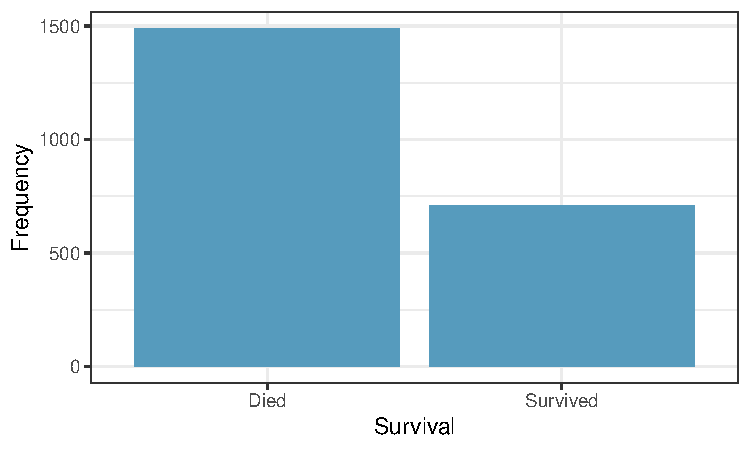
\includegraphics[width=0.45\textwidth]{2-2_categorical_data/figures/titanic_age_survival/titanic_bar}
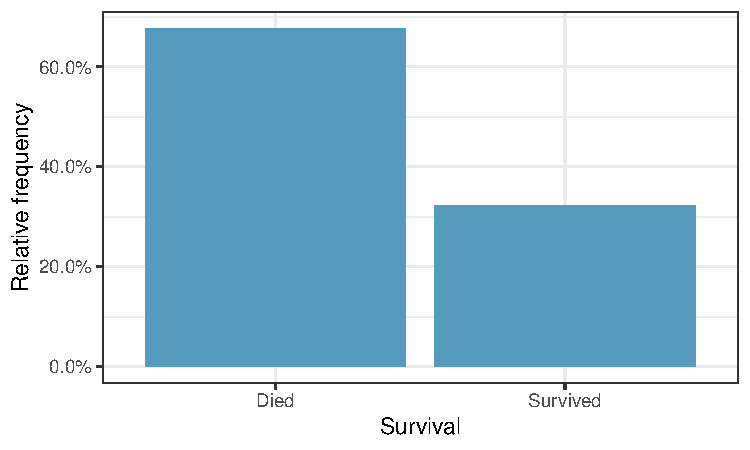
\includegraphics[width=0.45\textwidth]{2-2_categorical_data/figures/titanic_age_survival/titanic_rel_bar}
\end{center}

\dq{棒グラフとヒストグラムの違いは何か？}

\soln{{\tiny 棒グラフはカテゴリ変数の分布を表示するために使い、ヒストグラムは数値変数に使う。ヒストグラムのx軸は数直線であるため、棒の順序は変えられない。棒グラフではカテゴリをどの順序でも並べられる（ただし一部の順序の方が自然であり、特に順序変数の場合はそうである）。}}

\end{frame}

%%%%%%%%%%%%%%%%%%%%%%%%%%%%%%%%%%%%

\subsection{行比率と列比率}

%%%%%%%%%%%%%%%%%%%%%%%%%%%%%%%%%%%%

\begin{frame}
\frametitle{適切な比率の選択}

\dq{タイタニック号の乗客において、年齢と生存の間に関係があるように見えるか？}

\begin{center}
\begin{tabular}{l l cc r}
                               &          & \multicolumn{2}{c}{{生存}} \\
  \cline{3-4}
                               &          & 死亡   & 生存   & 合計 \\
  \cline{2-5}
\multirow{2}{*}{{年齢}}& 大人 & 1438  & 654      & 2092 \\
                               & 子供 & 52    & 57        & 109\\
  \cline{2-5}
                               & 合計 & 1490  & 711      &  2201 \\
  \cline{2-5}
\end{tabular}
\end{center}

この問いに答えるために行比率を調べる：

\begin{itemize}

\item 生存した大人の割合：654 / 2092 $\approx 0.31$ \\

\item 生存した子供の割合：57 / 109 $\approx 0.52$ \\

\end{itemize}

\end{frame}

%%%%%%%%%%%%%%%%%%%%%%%%%%%%%%%%%%%%

\subsection{2変数の棒グラフ}

%%%%%%%%%%%%%%%%%%%%%%%%%%%%%%%%%%%%

\begin{frame}
\frametitle{2変数の棒グラフ}

\begin{itemize}

\item \hl{積み上げ棒グラフ：}分割表の情報を度数で表示するグラフ。

\item \hl{並列棒グラフ：}同じ情報を棒を積み上げる代わりに横に並べて表示する。

\item \hl{正規化積み上げ棒グラフ：}分割表の情報を比率で表示するグラフ。

\end{itemize}

\end{frame}

%%%%%%%%%%%%%%%%%%%%%%%%%%%%%%%%%%%%

\begin{frame}

\dq{下の3つの図の違いは何か？}

\begin{center}
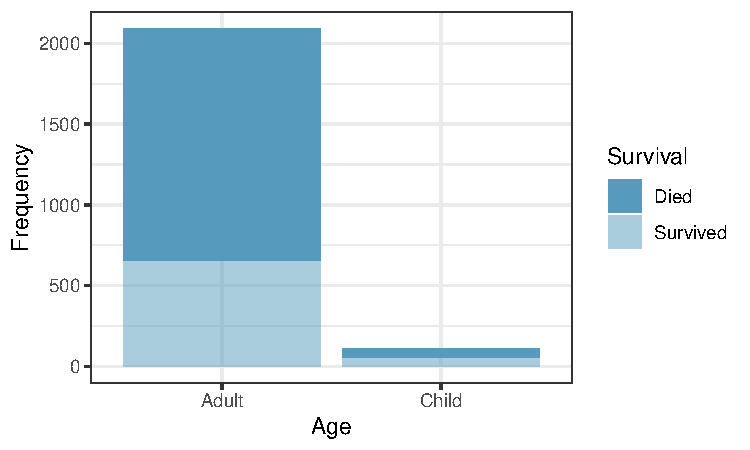
\includegraphics[width=0.42\textwidth]{2-2_categorical_data/figures/titanic_age_survival/titanic_seg_bar}
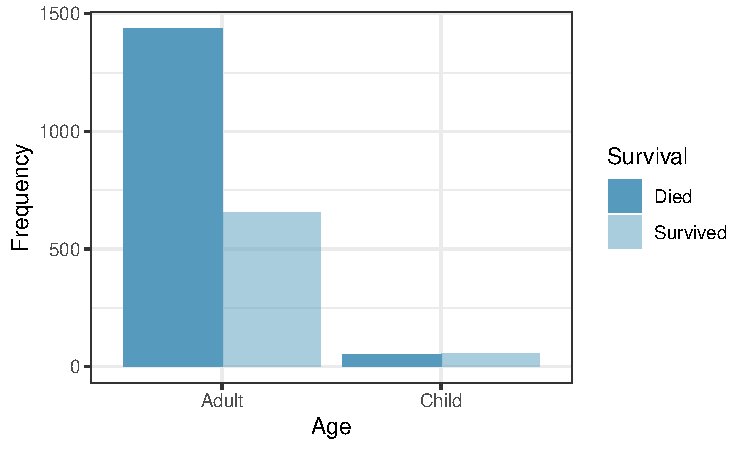
\includegraphics[width=0.42\textwidth]{2-2_categorical_data/figures/titanic_age_survival/titanic_seg_bar_dodge} \\
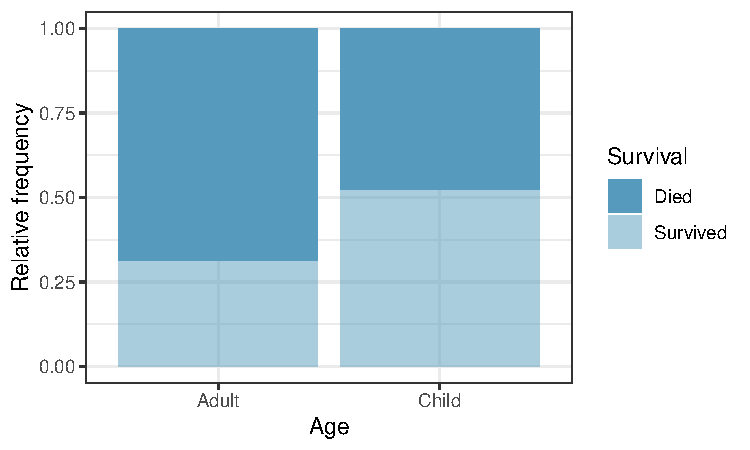
\includegraphics[width=0.42\textwidth]{2-2_categorical_data/figures/titanic_age_survival/titanic_rel_seg_bar}
\end{center}

\end{frame}

%%%%%%%%%%%%%%%%%%%%%%%%%%%%%%%%%%%%

\subsection{モザイクプロット}

%%%%%%%%%%%%%%%%%%%%%%%%%%%%%%%%%%%%

\begin{frame}
\frametitle{モザイクプロット}

\dq{下の2つの図の違いは何か？}

\begin{center}
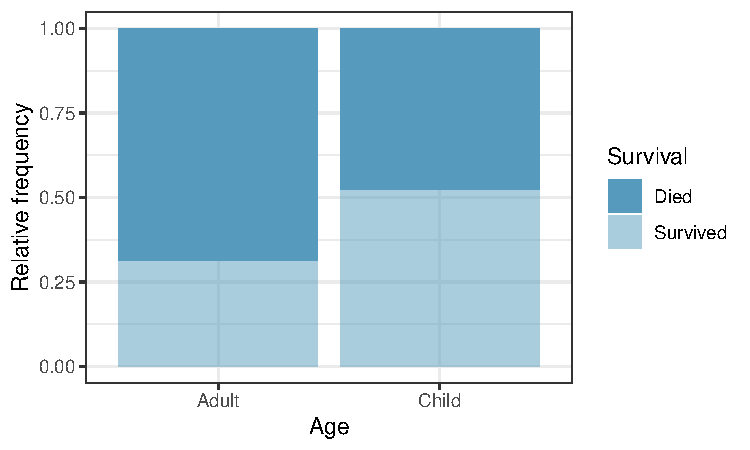
\includegraphics[width=0.47\textwidth]{2-2_categorical_data/figures/titanic_age_survival/titanic_rel_seg_bar}
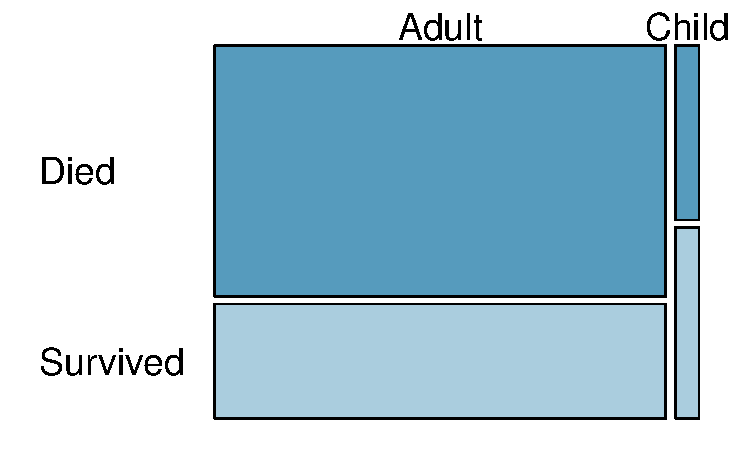
\includegraphics[width=0.47\textwidth]{2-2_categorical_data/figures/titanic_age_survival/titanic_mosaic}
\end{center}

\end{frame}

%%%%%%%%%%%%%%%%%%%%%%%%%%%%%%%%%%%%

\subsection{円グラフ}

%%%%%%%%%%%%%%%%%%%%%%%%%%%%%%%%%%%%

\begin{frame}
\frametitle{円グラフ}

\dq{哺乳類の種の割合が最も低い目（もく）はどれか分かるか？}

\vspace{-0.5cm}

\begin{center}

\includegraphics[width=0.4\textwidth]{2-2_categorical_data/figures/mammal_pie_chart/mammal_pie_chart}
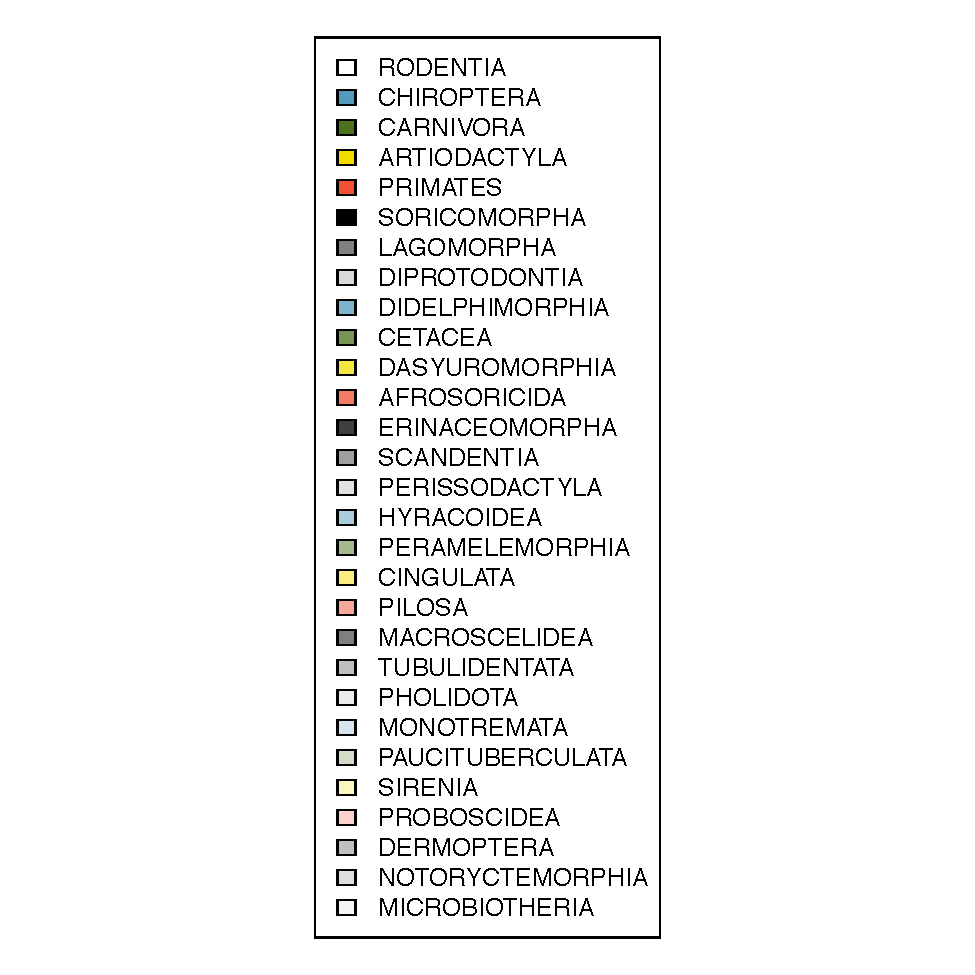
\includegraphics[width=0.2\textwidth]{2-2_categorical_data/figures/mammal_pie_chart/mammal_pie_chart_legend}
\end{center}

\ct{データ出典：\webURL{http://www.bucknell.edu/msw3}.}

\end{frame}


%%%%%%%%%%%%%%%%%%%%%%%%%%%%%%%%%%%%

\subsection{グループ間の数値データの比較}

%%%%%%%%%%%%%%%%%%%%%%%%%%%%%%%%%%%%

\begin{frame}
\frametitle{並列箱ひげ図}

\dq{学年と所属クラブ数の間に関係があるように見えるか？}

\begin{center}
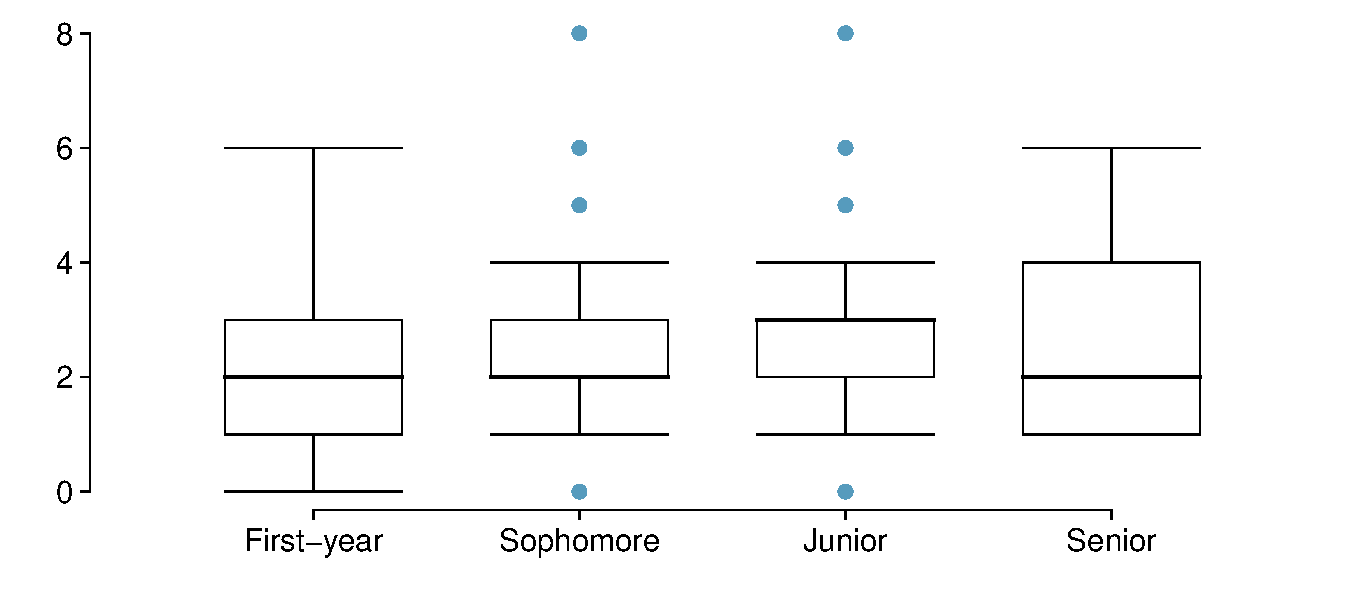
\includegraphics[width=\textwidth]{2-2_categorical_data/figures/year_clubs/year_clubs}
\end{center}

\end{frame}

%%%%%%%%%%%%%%%%%%%%%%%%%%%%%%%%%%%%
